\documentclass{beamer}
\usepackage{graphicx}
\usepackage{subcaption}
\usepackage{hyperref}
\usepackage{caption}
\usepackage{subcaption}

%Information to be included in the title page:
\title{Massively Parallel Evasion Attacks and the Pitfalls of Adversarial Retraining}
\author{Charles Meyers\inst{1} \and
Tommy L\"{o}fstedt\inst{2}  \and
Erik Elmroth\inst{3} }
\institute{ 
Department of Computing Science, Umeå University, Umeå, Sweden \email{cmeyers@cs.umu.se} \and 
\email{tommy@cs.umu.se} \and 
\email{eriks@cs.umu.se}
}
\date{25 October 2023}

\begin{document}

\frame{\titlepage}
\begin{frame}{Contributions}
    \begin{itemize}
    \small
    \item We provide an extensible and scalable code base for finding optimal attack configurations for a variety of attacks and defences.

    \item  We provide a method for faster attack generation for both benign (re-training) and adversarial circumstances, with easy extensibility to a variety of algorithms with large hyperparameter spaces including  models, defences, and attacks.
    
    \item We show that attack efficacy is uncorrelated with attack time and more dependent on the total perturbation distance and the step size at each iteration.

    \item We show that, the relationship between step size, perturbation size, and false confidence is highly complex, has a large hyperparameter space, and a product of both the model and the data set and that characterizing the feasible space is critical to generalized robustness.

    \item Using a strong adversary as determined by massively parallel tests, we found that adversarial retraining was impractical in terms of both compute time and benign model accuracy against a strong adversary on a variety of binary datasets.
    
\end{itemize}
\end{frame}
\begin{frame}{Datasets}
    \begin{itemize}
        \item \textbf{Generated Data:} Normally distributed data with $n$ samples and $p$ dimensions, linearly separable. Up to $10^6$ samples.
        \item \textbf{KDD-NSL:} Updated version of the KDD 99 dataset to remove repeated rows. 10s of features and 1000s of samples. \cite{kdd-nsl}
        \item \textbf{Truthseeker:} Bot-net data collected via the Twitter API. 10s of features and 10s of thousands of samples. \cite{truthseeker}
        
    \end{itemize}
\end{frame}

\begin{frame}{Models}
    A support vector machine is trained by solving the Lagrange dual problem~\cite{cortes1995support},
\begin{equation}
    \textrm{max}_{c_1,\ldots,c_n}
    \sum_{i = 1}^n c_i - \frac{1}{2} \sum_{i = 1}^n \sum_{j = 1}^n y_i c_i \langle x_i, x_j \rangle y_j c_j
    \label{eq:linear_svm}
\end{equation}
$$
    \textrm{subject to } \sum_{i = 1}^n c_i y_i = 0 \textrm{\quad and\quad} 0 \leq c_i \leq \frac{1}{2n\lambda}, \forall i,
$$
where $x_1,\ldots,x_n$ is the set of training examples, $y_1,\ldots,y_n$ are the training labels for the $n$ samples, the $c_i$ are the dual variables found during training, and $\lambda$ is a regularization parameter that controls the complexity of the decision boundary by penalizing wrong classifications. Solving this quadratic problem requires at least $O(n^2)$ dot products, making it computationally expensive for large data-sets.
\end{frame}

\begin{frame}{Attack: Projected Gradient Descent}
The \textbf{PGD Attack} is defined by the iteration scheme:
$$
    x^{(k+1)} = P\big(x^{(k)} + \eta^{(k)} \nabla f(x^{(k)})\big),
$$
where $x^{(k)}$ is the adversarial example at iteration $k = 1,\ldots,N$, the $N$ is the number of iterations, $P(x)$ is a projection of $x$ onto a convex set (e.g., a norm ball in the feature space) with radius $d_{max}$ (chosen by the experimenter), $\eta^{(k)}$ is the step size in each iteration, and $f(x^{(k)})$ is the original model function at iteration $k$. An attack thus takes ascent steps in the direction of the loss gradient, attempting to maximize the loss of the attacked model, with the projection step as a means to adhere to any other constraints.
\end{frame}

\begin{frame}{Adversarial Retraining}
    Adversarial retraining inherits the time complexity of both the model and the attack above such that the complexity is
$$
    O(n^2p),
$$
before actually creating the retrained model, which has $2n$ samples, giving us the complexity
$$
    O(n^2p) + O\big((2n)^2\big) = O(n^2p)
$$
which will add significant training time to the model (already measured in hours or days) with the unintended side effect of reducing benign accuracy~\cite{stutz2019confidence}.
\end{frame}

\begin{frame}{Pipeline}
  \begin{figure*}
\centering
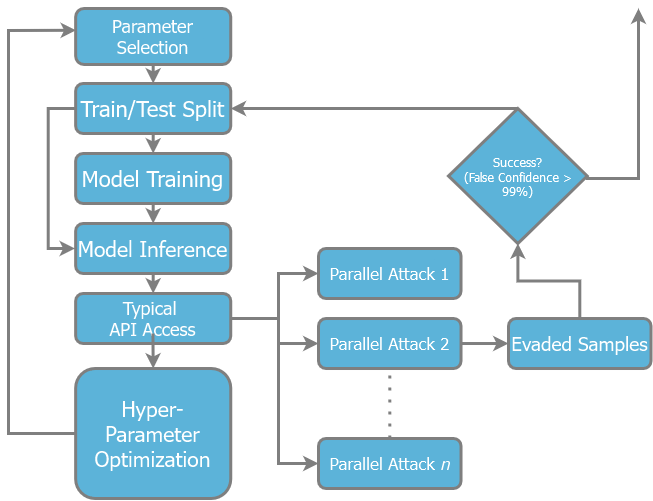
\includegraphics[width=\textwidth]{ppgd.png}

\label{fig:attack_framework}
\caption{Massively Parallel Attack and Re-training Framework.  This depicts our experimental pipeline wherein we build KSVMs with various kernels, run several attacks in parallel, and then evaluate the attacked samples on the models. Optionally, we collect highly confident false examples for adversarial retraining.}
\end{figure*}
\end{frame}

\begin{frame}{Methods}
\small
We dedicated one core to each attack and tested a large number of hyperparameters at the same time using `joblib'\footnote{\href{https://joblib.readthedocs.io}{https://joblib.readthedocs.io}}. We used the \texttt{optuna}~\cite{optuna} framework for handling scheduling\footnote{\href{https://optuna.readthedocs.io}{https://optuna.readthedocs.io}}, hydra\footnote{\href{https://hydra.cc}{https://hydra.cc}} for hyperaparamater configuration management, and dvc\footnote{\href{https://dvc.org}{https://dvc.org}} to track results and guarantee reproducibility.
  By using a massively parallel \cite{optuna} implementation, we were able to generate tens of thousands of strong examples from one-thousand input-output pairs in a way that extends to other attacks, frameworks (\textit{e.g.}~MXNet, Pytorch, Keras, Tensorflow), and defences (\textit{e.g.}~ART). Our implementation\footnote{\href{https://github.com/simplymathematics/deckard}{Our Github Repository}} allocates one core per process and runs them in series if there are more processes queued than available cores. All generated models, data, and results are stored to disk, as well as in an sqlite database, all specified in a single configuration file, allowing for arbitrary divisions of the evaluation pipeline across any number of diverse and distributed machines.
\end{frame}

\begin{frame}{Model Performance vs Database Size}
  \begin{figure}
    \centering
    \begin{subfigure}{.45\textwidth}
      \centering
      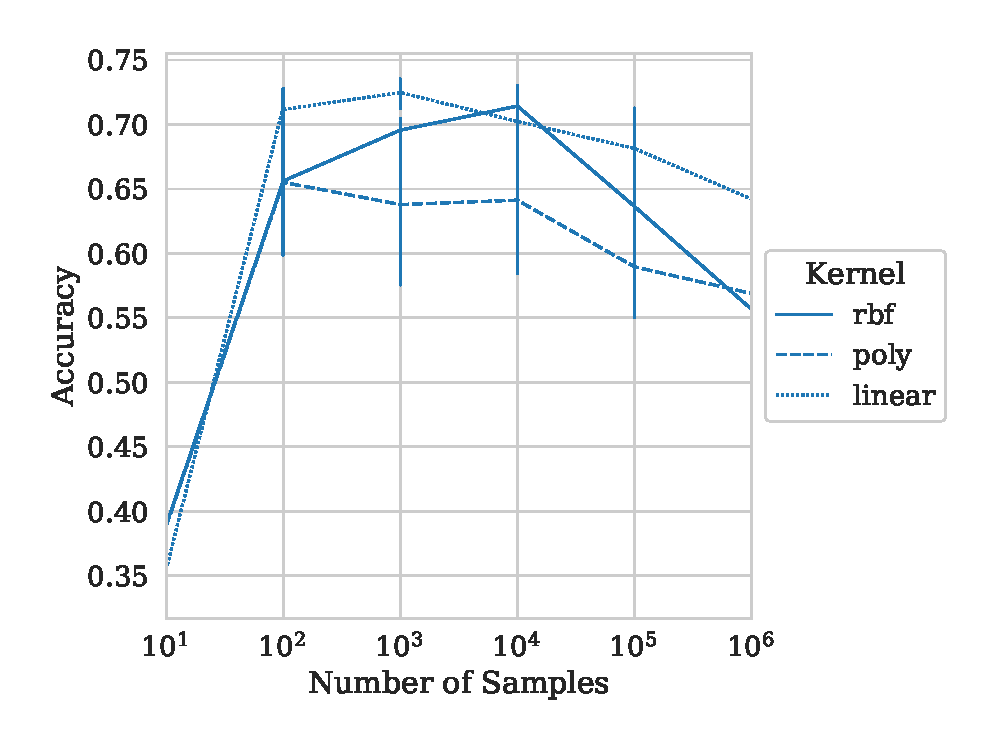
\includegraphics[width=\textwidth]{./generated/accuracy_vs_samples.eps}
      \caption{Model Performance vs Database Size}
    \end{subfigure}
    \hfill
    \begin{subfigure}{.45\textwidth}
      \centering
      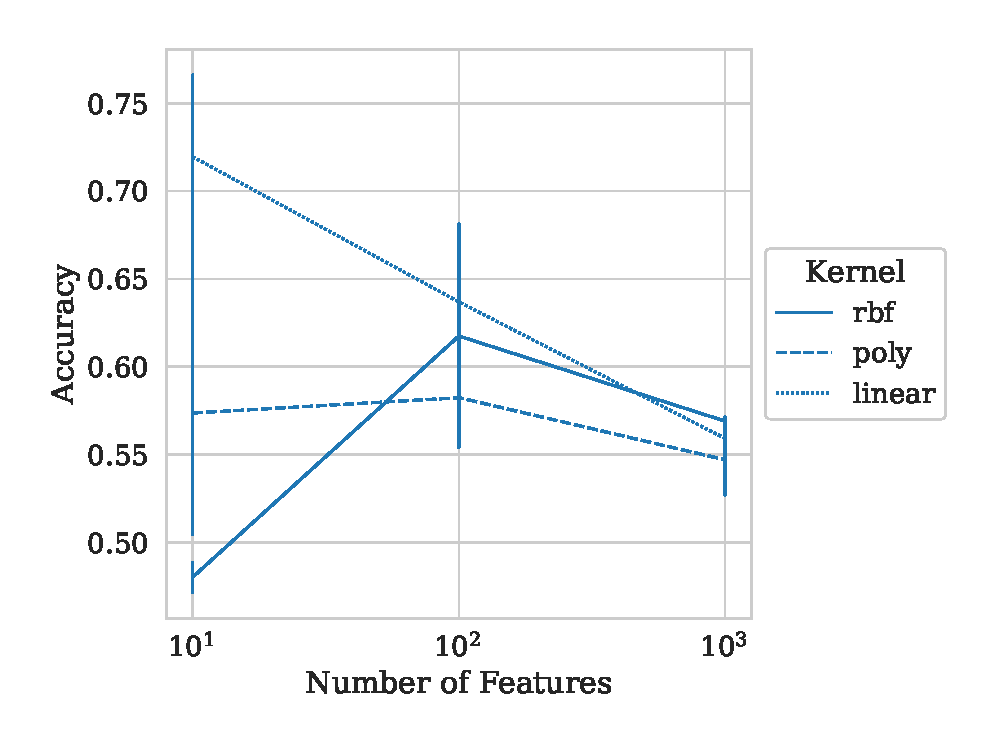
\includegraphics[width=\textwidth]{./generated/accuracy_vs_features.eps}
      \caption{Model Performance vs Feature Space}
    \end{subfigure}
  \end{figure}
\end{frame}

\begin{frame}{Training and Attack Times vs Database Size}
  \begin{figure}
    \centering
    \begin{subfigure}{.45\textwidth}
      \centering
      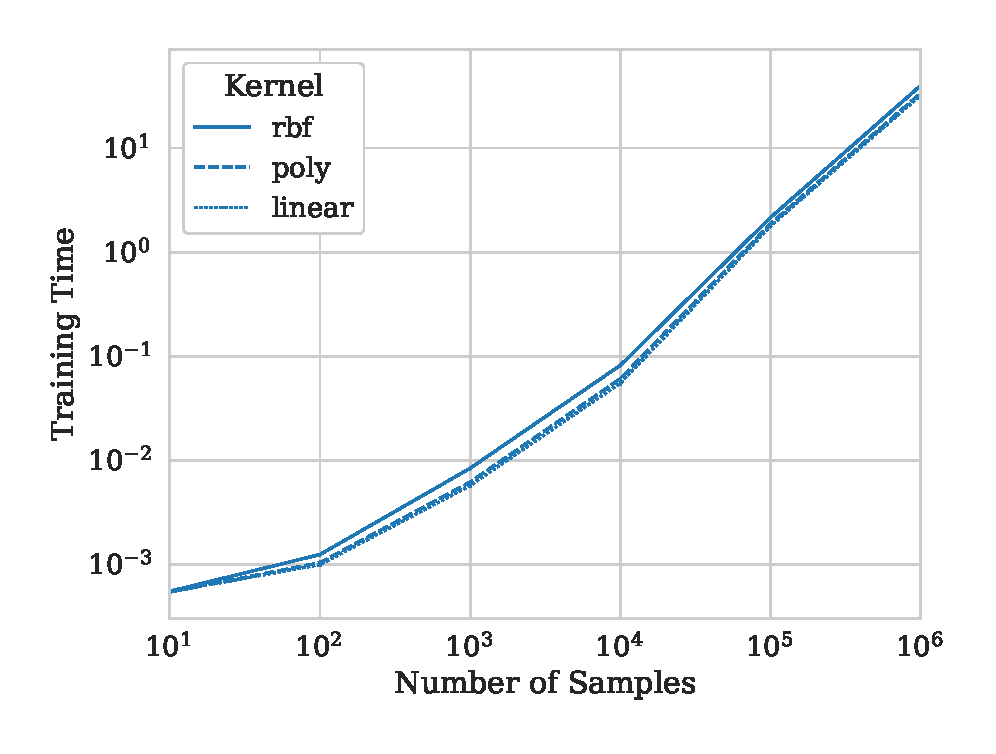
\includegraphics[width=\textwidth]{./generated/train_time_vs_samples.eps}
      \caption{Training and Attack Times vs Database Size}
    \end{subfigure}
    \hfill
    \begin{subfigure}{.45\textwidth}
      \centering
      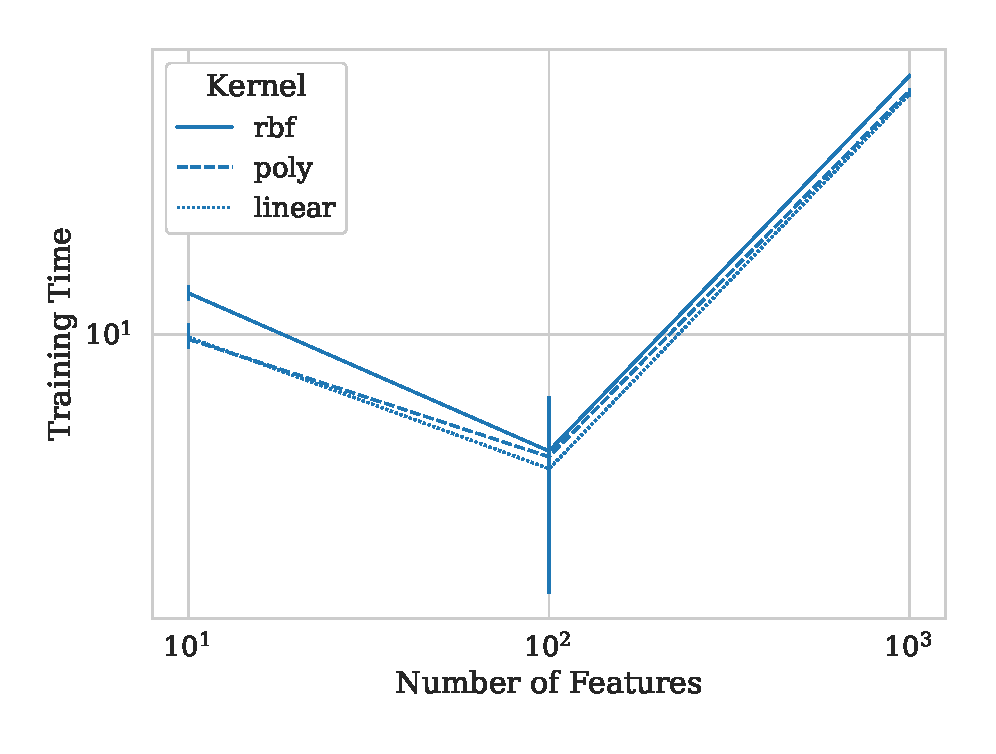
\includegraphics[width=\textwidth]{./generated/train_time_vs_features.eps}
      \caption{Training and Attack Times vs Feature Space}
    \end{subfigure}
  \end{figure}
\end{frame}


\begin{frame}{Attack Parameters vs Accuracy}
  \begin{figure}
    \centering
    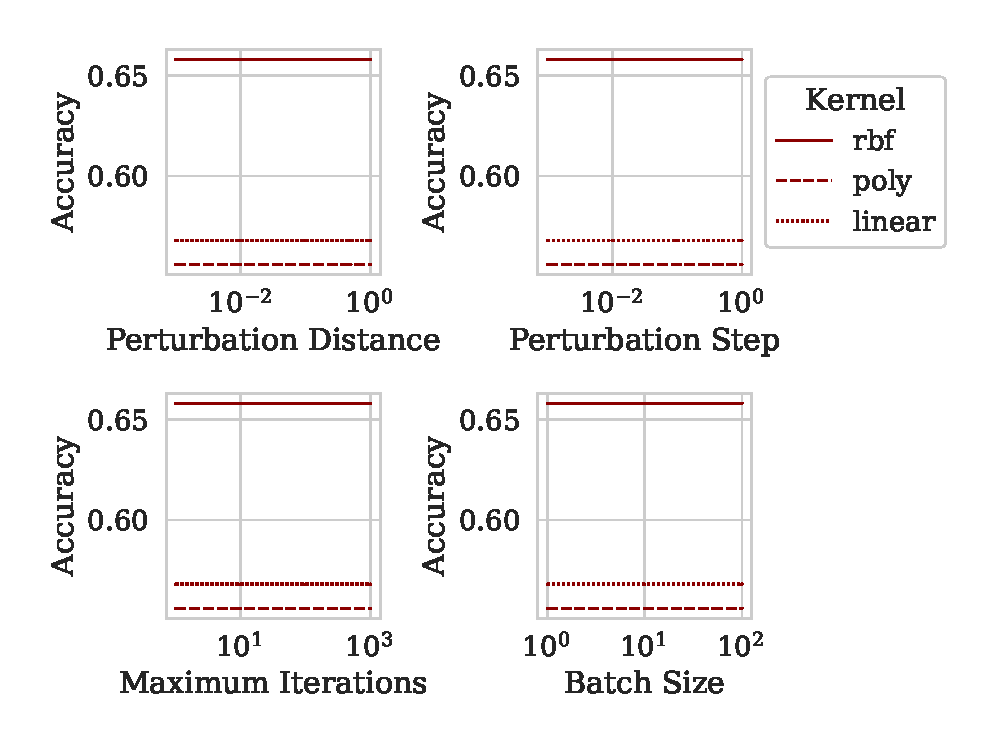
\includegraphics[width=.75\textwidth]{./generated/accuracy_vs_attack_parameters.eps}
    \caption{Attack Parameters vs Accuracy}
  \end{figure}
  \label{fig:attack_accuracy}
\end{frame}

\begin{frame}{Attack Parameters vs Time}
  \begin{figure}
    \centering
    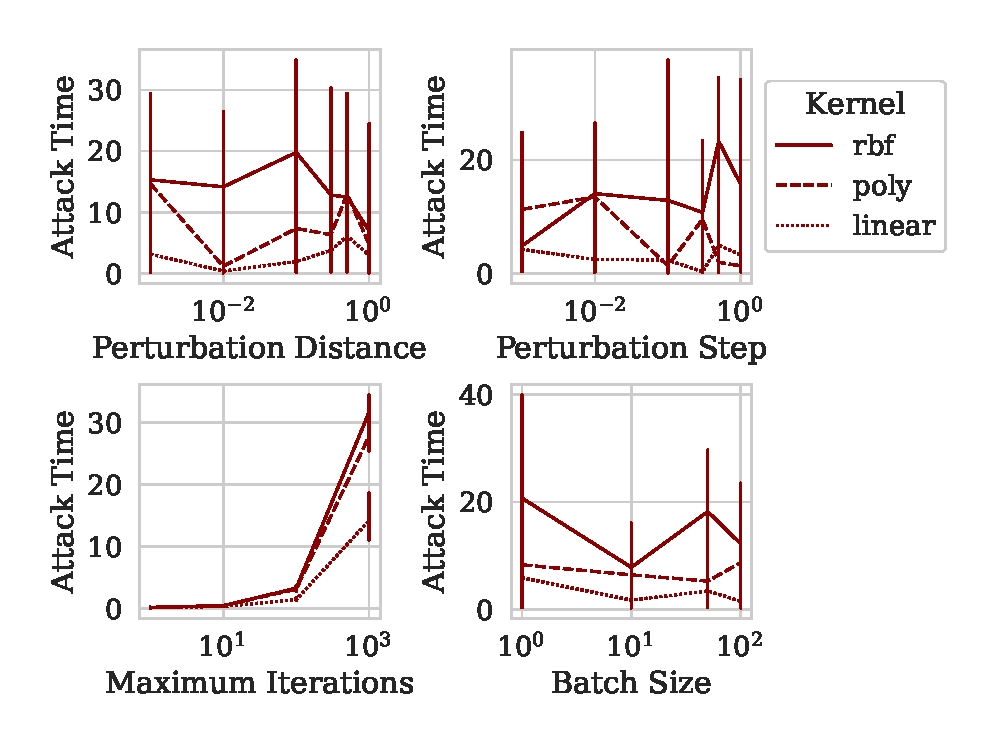
\includegraphics[width=.75\textwidth]{./generated/train_time_vs_attack_parameters.eps}
    \caption{Attack Parameters vs Time}
  \end{figure}
\end{frame}


\begin{frame}{Adversarial Retraining: Accuracy over Retraining Cycles}
  \begin{figure}
    \centering
    \begin{subfigure}[b]{0.45\textwidth}
      \centering
      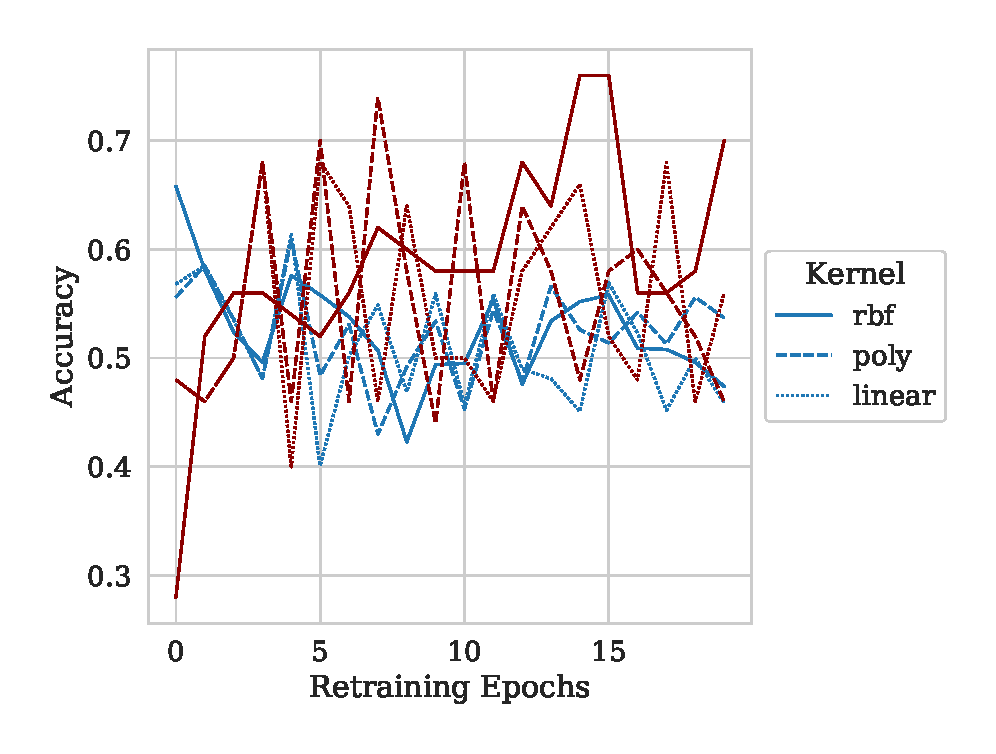
\includegraphics[width=\textwidth]{./generated/retrain_accuracy.eps}
      \caption{Adversarial Retraining: Accuracy over Retraining Cycles}
    \end{subfigure}
    \centering
    \begin{subfigure}[b]{0.45\textwidth}
      \centering
      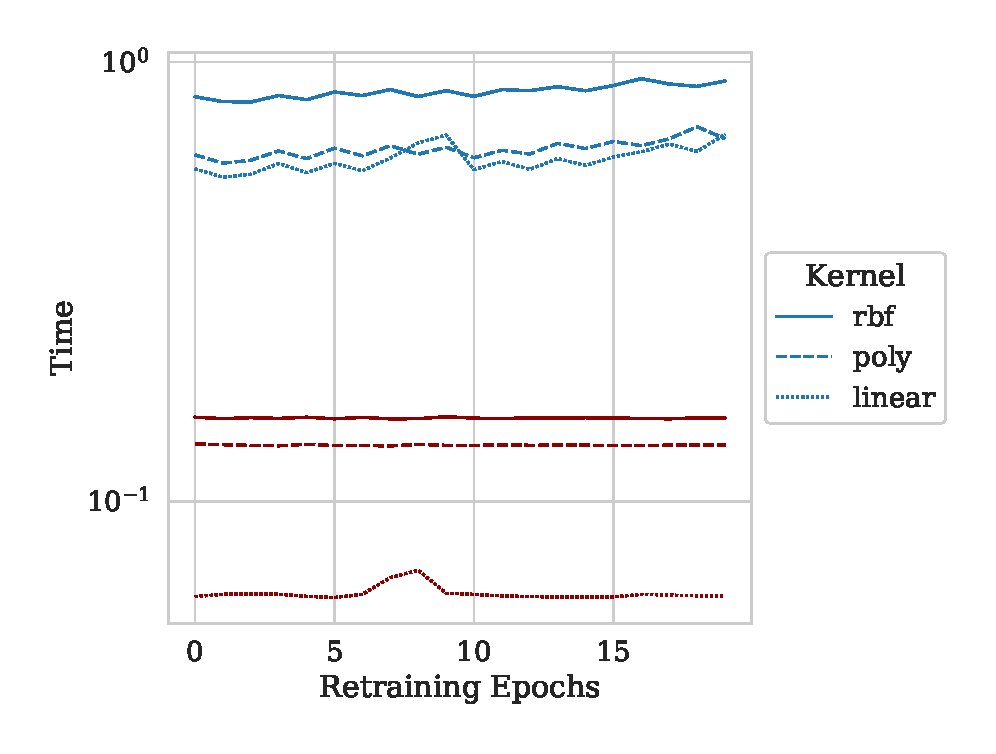
\includegraphics[width=\textwidth]{./generated/retrain_time.eps}
      \caption{Adversarial Retraining: Training and Attack Times}
    \end{subfigure}
  \end{figure}
\end{frame}

\begin{frame}{False Negative Classifications Before and After Retraining}
  \begin{figure}
    \centering
    \begin{subfigure}[b]{0.45\textwidth}
      \centering
      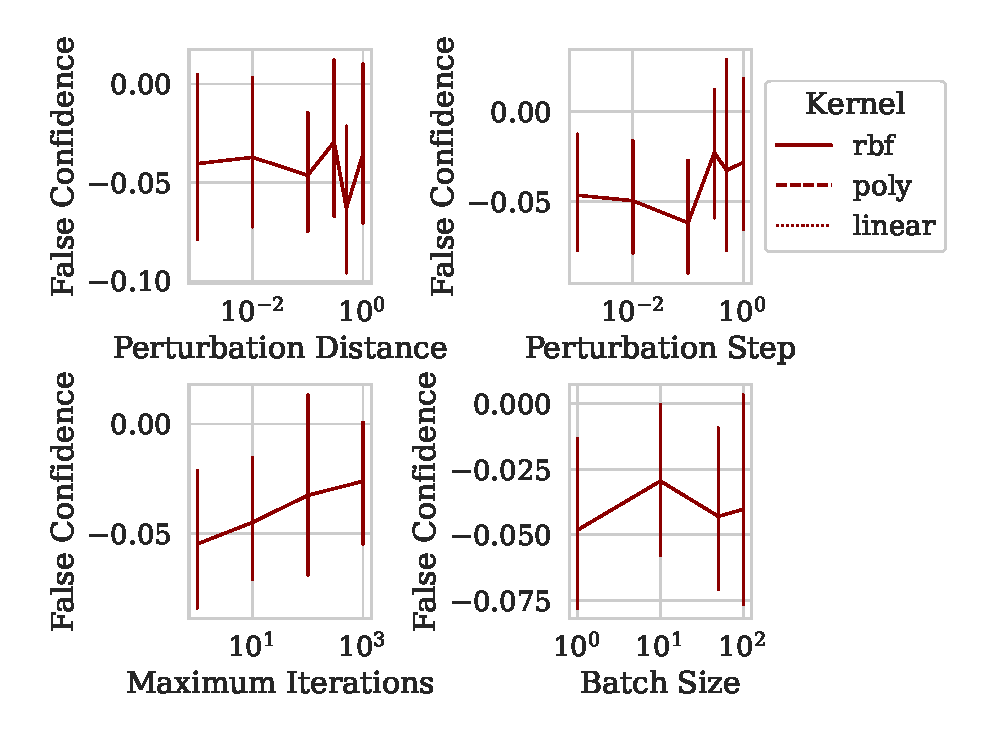
\includegraphics[width=\textwidth]{./generated/confidence_vs_attack_parameters.eps}
      \caption{False Negative Classifications Before Retraining}
    \end{subfigure}
    \centering
    \begin{subfigure}[b]{0.45\textwidth}
      \centering
      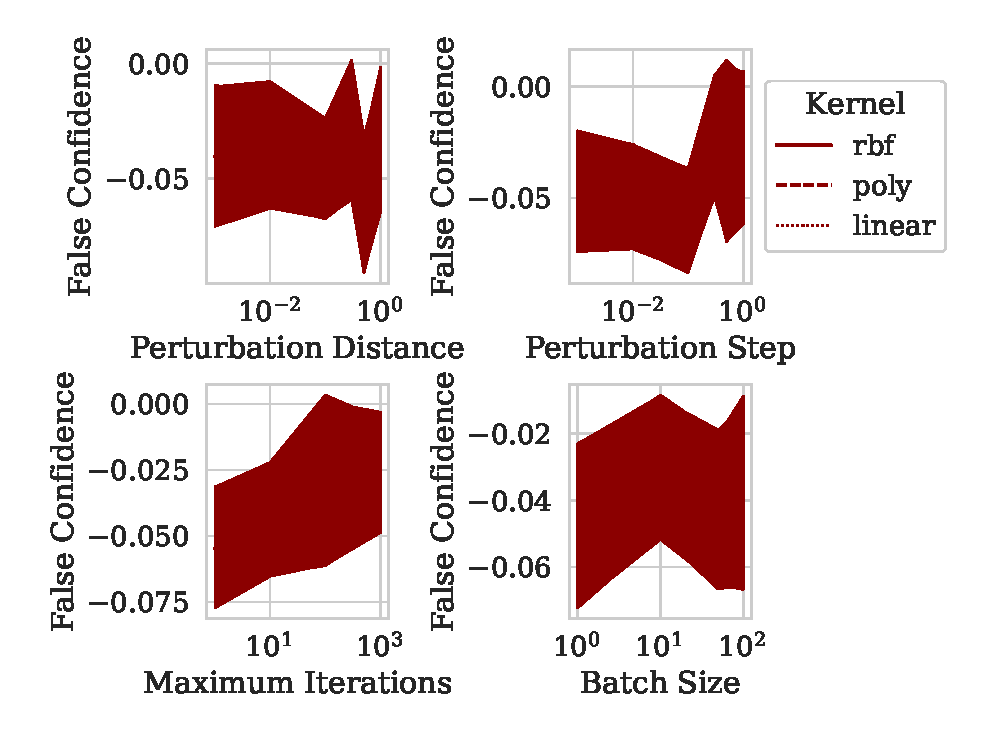
\includegraphics[width=\textwidth]{./generated/retrain_confidence_vs_attack_parameters.eps}
      \caption{False Negative Classifications After Retraining}
    \end{subfigure}
  \end{figure}
\end{frame}


\begin{frame}{Accuracy and Robustness}
  Much research has been devoted to the apparent trade-off between robustness and benign accuracy and we see signs of it across all of our experiments. 
  \begin{itemize}
      \item The second experiment confirmed an inverse relationship between robustness and model accuracy.
      \item Even when AT is able to perfectly classify adversarial examples in the new training set, average error in the benign circumstance increased from 0.02\% to roughly 50\%.
      \item The adversarial accuracy against strong attacks increased, but at a substantial cost to adversarial accuracy. This would be catastrophic in safety- or security-critical settings.
  \end{itemize}  
\end{frame}

\begin{frame}{Attack Time and Efficacy}
  Since PGD is iterative, we examined how increasing the raw compute time changes attack efficacy. 
  \begin{itemize}
      \item there is no general relationship between attack time and error when we examine the entire attack space.
      \item The attacks that produce the largest errors are more dependent on hyper-parameter choice than raw processing time. 
      \item  there are many examples where attack error was maximized with a small number of iterations
      \item That is, a 'good' attack converges on strong adversarial examples quickly.
  \end{itemize}
\end{frame}

\begin{frame}{Critical Space}
  To reliably evaluate a model, we must look at how it performs across many attacks, so we measured both error and false confidence for the entire attack space. 
  \begin{itemize}
      \item We see that increasing either step size or perturbations tends to increase loss with a minimal perturbation size required by a given model and data-set.
      \item  In addition, we found that there is a minimum perturbation value for effective attacks, dependent on model and data.
      \item the relationship between loss, step size, batch size, and iterations is complex and requires tuning
  \end{itemize}
  
\end{frame}



\begin{frame}{KDD-NSL}
    \begin{figure}
     \centering
     \begin{subfigure}{0.4\textwidth}
         \centering
         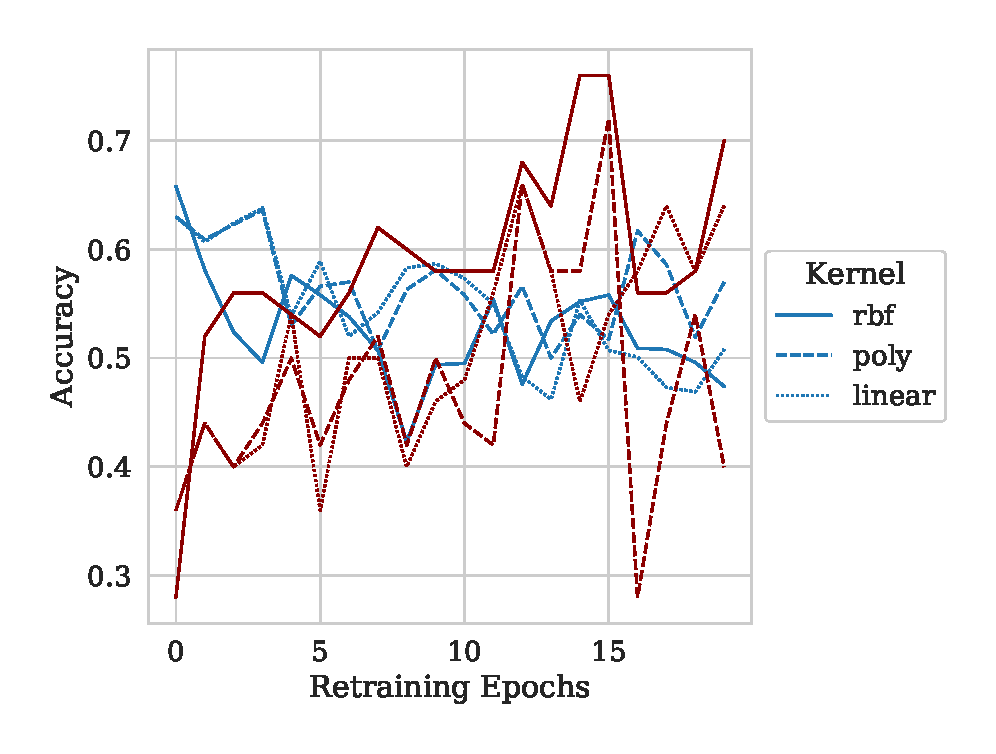
\includegraphics[width=\textwidth]{./kdd-nsl/retrain_accuracy.eps}
         \caption{Accuracy After Retraining}
     \end{subfigure}
     \hfill
     \begin{subfigure}{0.4\textwidth}
         \centering
         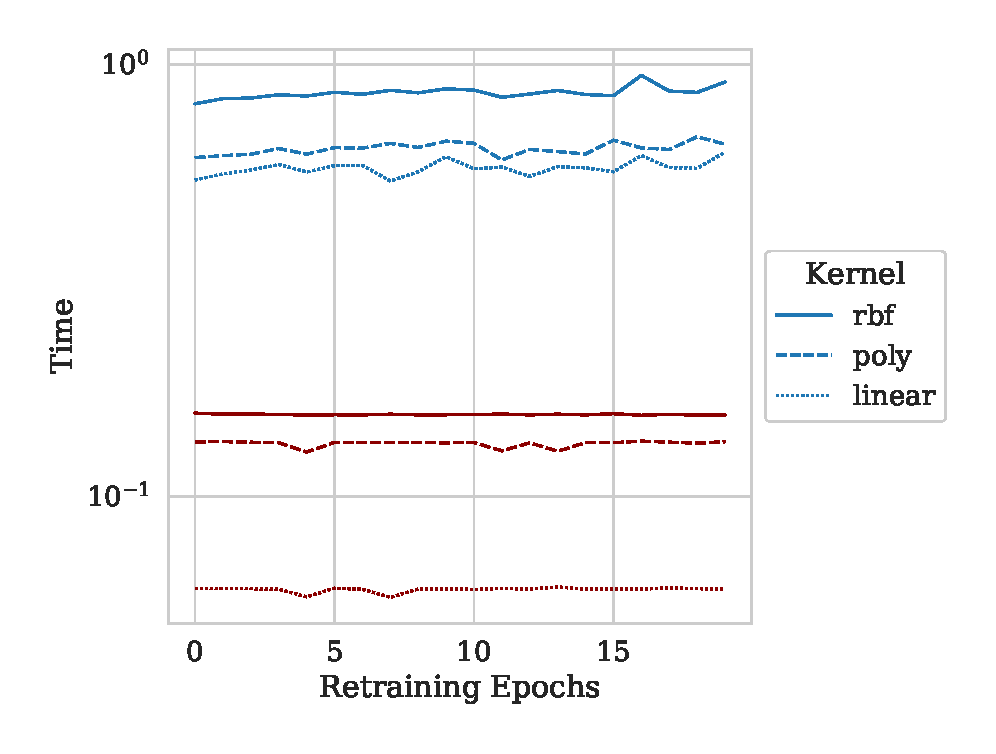
\includegraphics[width=\textwidth]{./kdd-nsl/retrain_time.eps}
         \caption{Retraining Time}
     \end{subfigure}
     \hfill
     \begin{subfigure}{0.4\textwidth}
         \centering
         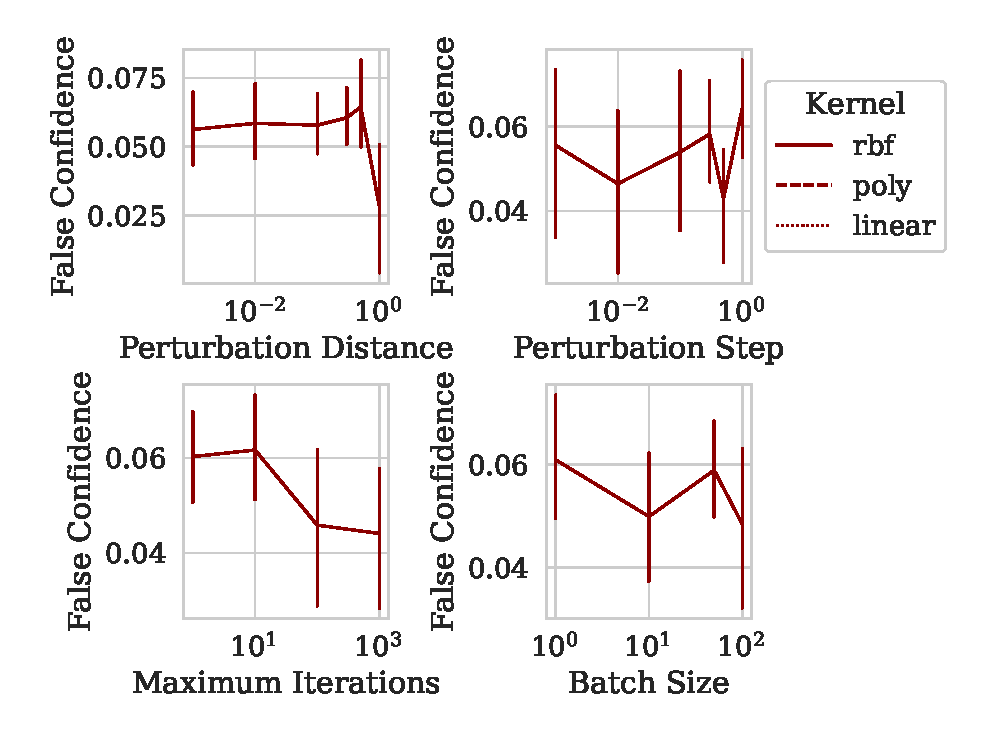
\includegraphics[width=\textwidth]{./kdd-nsl/confidence_vs_attack_parameters.eps}
         \caption{Before Retraining}
     \end{subfigure}
     \hfill
     \begin{subfigure}{0.4\textwidth}
         \centering
         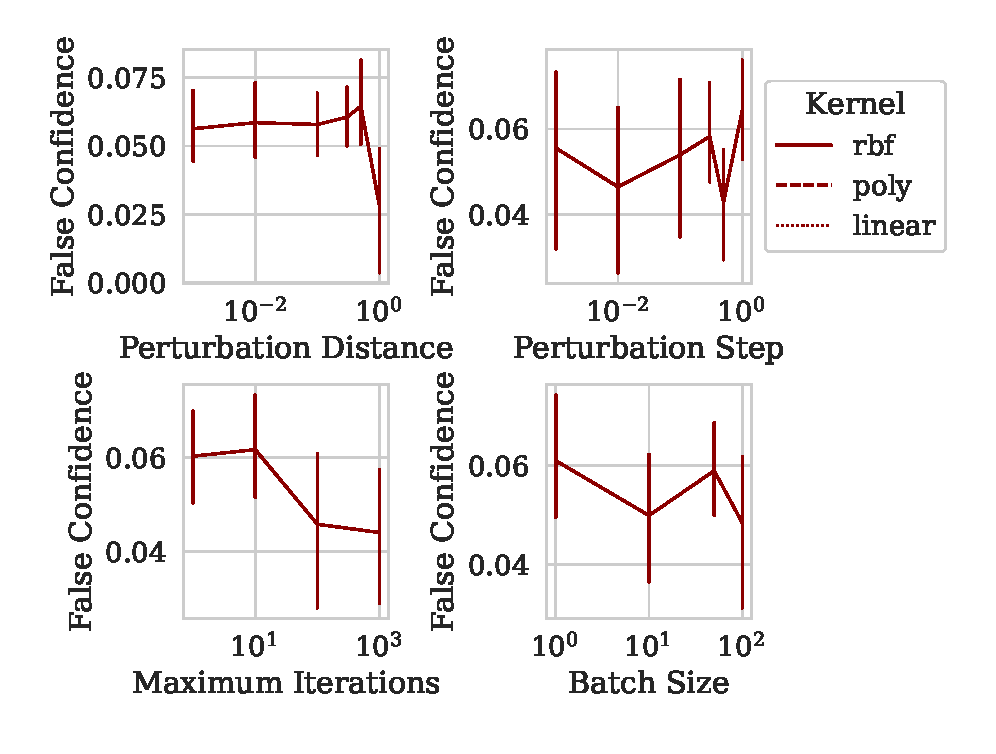
\includegraphics[width=\textwidth]{./kdd-nsl/retrain_confidence_vs_attack_parameters.eps}
         \caption{After Retraining}
     \end{subfigure}
     
     \label{fig:kdd-nsl}
\end{figure}
\end{frame}

\begin{frame}{Truthseeker}
    \begin{figure}
     \centering
     \begin{subfigure}{0.4\textwidth}
         \centering
         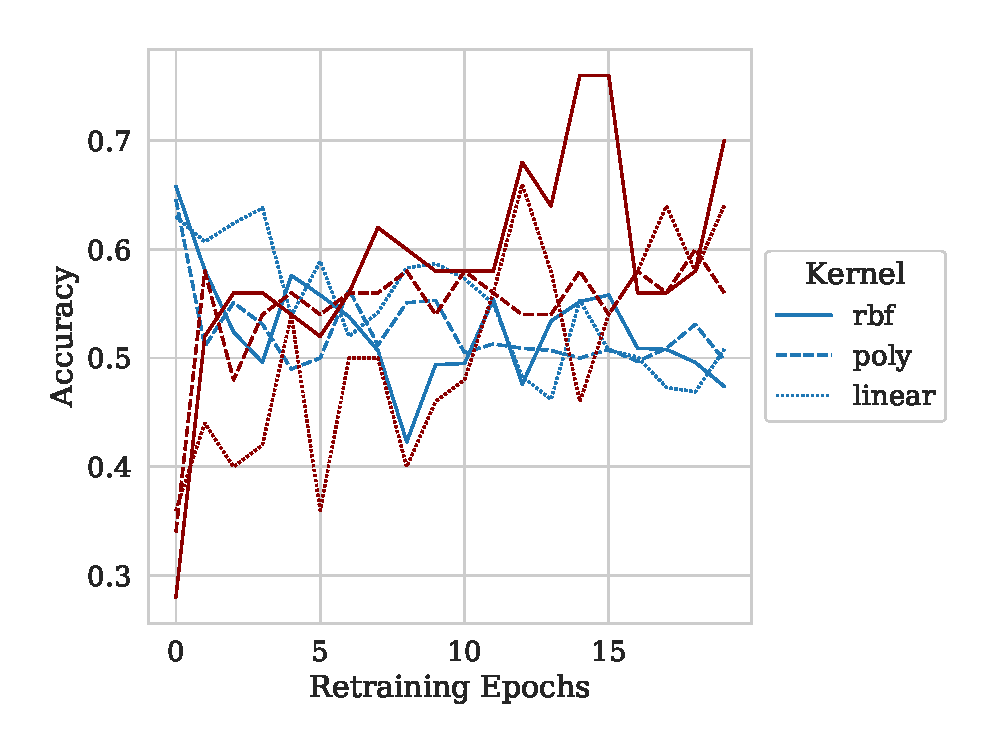
\includegraphics[width=\textwidth]{./truthseeker/retrain_accuracy.eps}
         \caption{Accuracy After Retraining}
     \end{subfigure}
     \hfill
     \begin{subfigure}{0.4\textwidth}
         \centering
         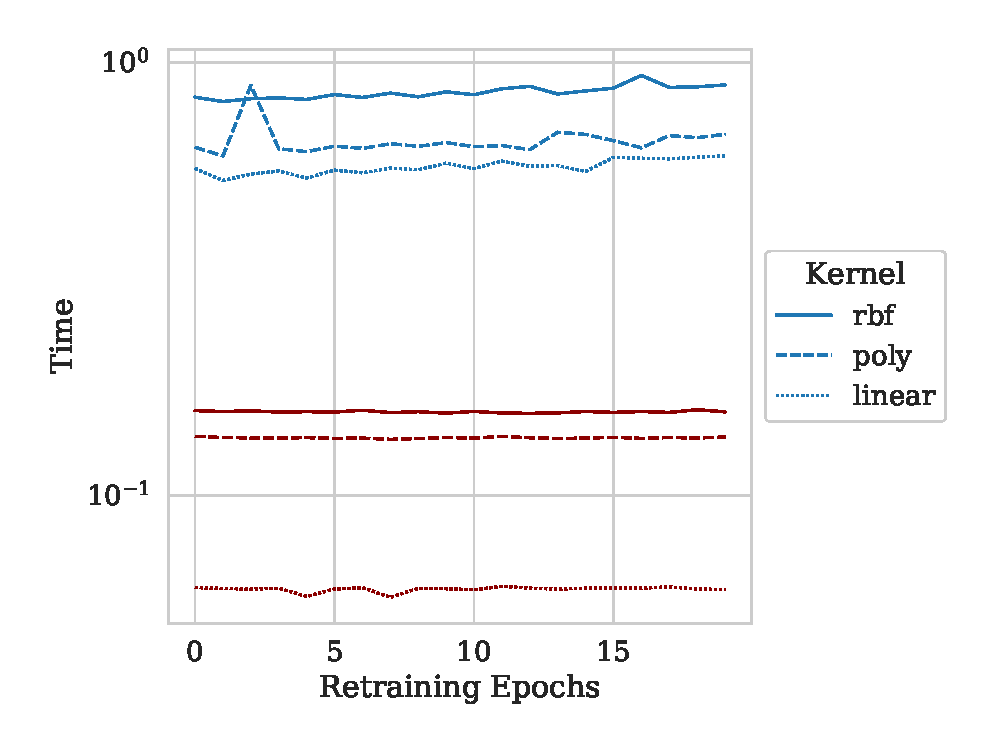
\includegraphics[width=\textwidth]{./truthseeker/retrain_time.eps}
         \caption{Retraining Time}
     \end{subfigure}
     \hfill
     \begin{subfigure}{0.4\textwidth}
         \centering
         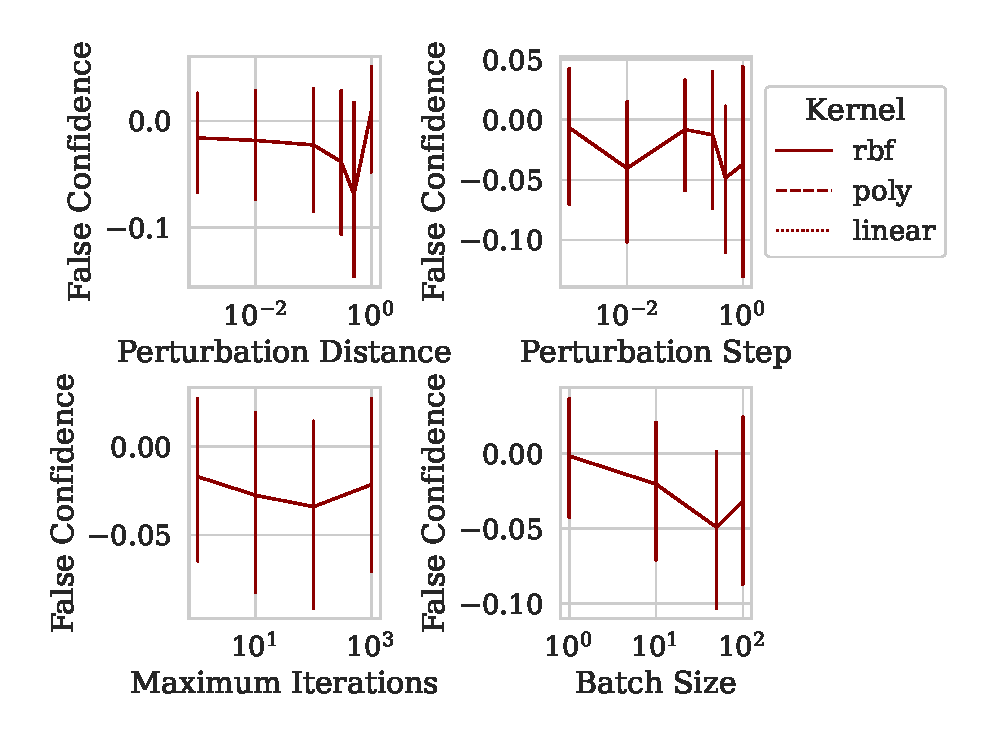
\includegraphics[width=\textwidth]{./truthseeker/confidence_vs_attack_parameters.eps}
         \caption{Before Retraining}
     \end{subfigure}
     \hfill
     \begin{subfigure}{0.4\textwidth}
         \centering
         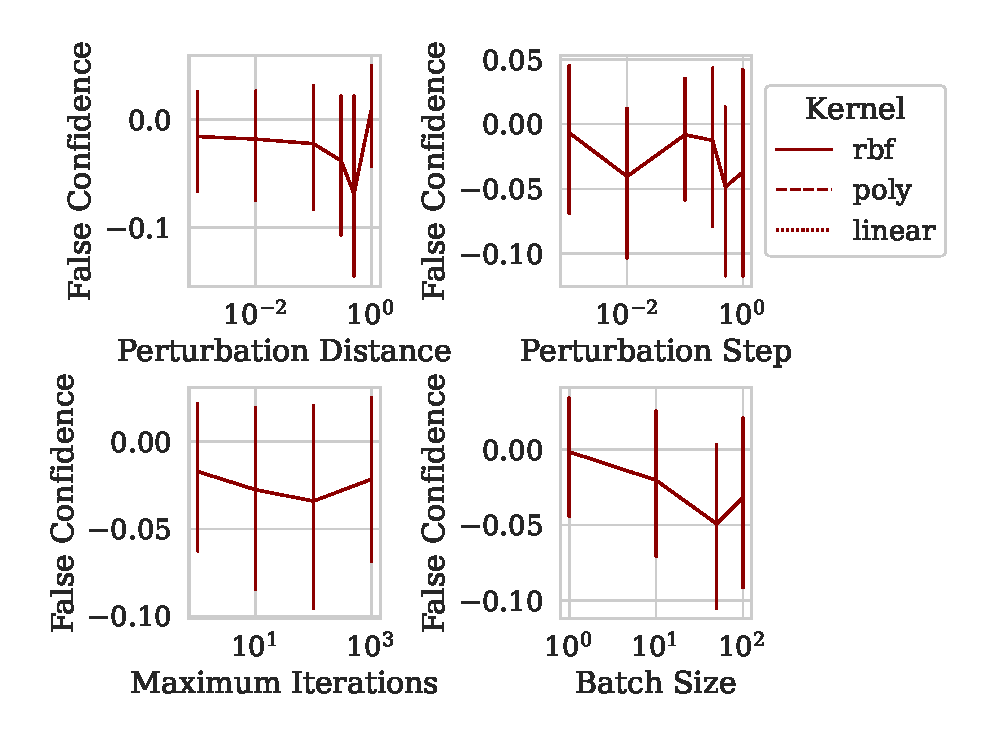
\includegraphics[width=\textwidth]{./truthseeker/retrain_confidence_vs_attack_parameters.eps}
         \caption{After Retraining}
     \end{subfigure}
     \hfill
     \label{fig:truthseeker}
\end{figure}
\end{frame}

\begin{frame}{Conclusion}
  In conclusion, our findings suggest that adversarial retraining is not suitable for real-time, safety-critical, or security-sensitive applications of KSVMs. We raise serious concerns about the hope of any polynomial-time model builder to defend against an adversary that consistently succeeds in more-or-less constant time, despite many rounds of adversarial retraining. Furthermore, we show this to be true on generated data, system process data, and social media data.
\end{frame}

\begin{frame}{Bibliography}
\scriptsize
\bibliographystyle{splncs04}
\bibliography{bibliography}
\end{frame}

\begin{frame}{Further Work}
    \begin{itemize}
        \item Finding an optimal attack via learning rate optimization
        \item Examining linear-time models
        \item Comparative attack and defence metric to quickly reject bad defences or ineffective attacks
        \item Other thoughts?
    \end{itemize}
\end{frame}

\end{document}
